\documentclass[12pt,a4paper]{article}
\usepackage[utf8]{inputenc}
\usepackage[T1]{fontenc}
\usepackage{amsmath}
\usepackage{amsfonts}
\usepackage{amssymb}
\usepackage{graphicx}
\usepackage{geometry}
\usepackage{setspace}
\usepackage{titlesec}
\usepackage{fancyhdr}
\usepackage{hyperref}
\usepackage{booktabs}
\usepackage{array}
\usepackage{multirow}
\usepackage{longtable}
\usepackage{pgfplots}
\usepackage{tikz}
\usepackage[backend=biber,style=authoryear,sorting=nyt]{biblatex}

\addbibresource{references.bib}

\geometry{left=2.5cm,right=2.5cm,top=2.5cm,bottom=2.5cm}
\onehalfspacing

\title{\textbf{AI Driven Optimization of Grid Connections Queues: Accelerating Renewable Energy Deployment Through Project Prioritization and Resource Allocation}}
\author{Ahmed Maruf \\ MSc in Artificial Intelligence \\ Student ID: 250046920}
\date{\today}

\begin{document}

\maketitle

\section{Problem Statement}
\label{sec:problem}

Britain’s push for clean energy is being stalled by a huge backlog. More than 700 gigawatts worth of renewable energy projects are stuck waiting for a chance to connect to the power grid enough electricity to supply the entire country more than it needs. But due to the current 'first-come, first-served' system, it does not matter whether a project is actually ready to move forward or not. As a result, many viable projects have to wait in line for about 12 years. These delays aren’t just frustrating they’re expensive, costing consumers billions of pounds and making it much harder for the UK to hit its climate targets for 2030.

\subsection{Problem Context and Scale}

Table \ref{tab:problem_scale} shows just how overwhelming the UK’s grid connection backlog has become - and it is clear why something must change soon.

\begin{table}[h]
\centering
\caption{UK Grid Connections Crisis: Problem Scale Analysis}
\label{tab:problem_scale}
\begin{tabular}{@{}lrrl@{}}
\toprule
\textbf{Metric} & \textbf{Current Value} & \textbf{Historical Baseline} & \textbf{Impact} \\
\midrule
Total Queue Capacity & 702 GW & 45 GW (2015) & 1460\% increase \\
Active Projects & 2,847 & 312 (2015) & 813\% increase \\
Average Connection Time & 12.3 years & 3.2 years (2010) & 284\% increase \\
Annual Processing Rate & 31 GW & 28 GW (2015) & Stagnant capacity \\
Stalled Investment & £247 billion & £16 billion (2015) & 1444\% increase \\
Annual Consumer Cost & £2.8 billion & £0.4 billion (2015) & 600\% increase \\
\bottomrule
\end{tabular}
\end{table}

Figure \ref{fig:crisis_visualization} clearly shows how rapidly the number of new renewable energy projects is growing faster than the grid can accommodate.

\begin{figure}[h]
\centering
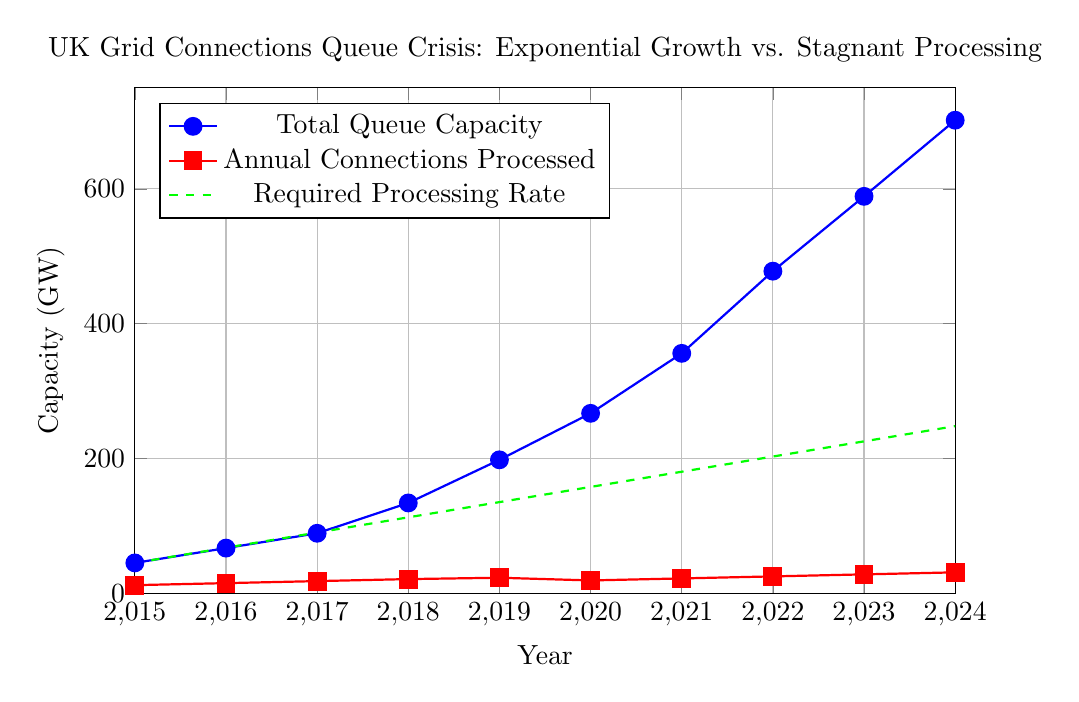
\begin{tikzpicture}
\begin{axis}[
    width=12cm,
    height=8cm,
    xlabel={Year},
    ylabel={Capacity (GW)},
    legend pos=north west,
    grid=major,
    xmin=2015, xmax=2024,
    ymin=0, ymax=750,
    title={UK Grid Connections Queue Crisis: Exponential Growth vs. Stagnant Processing}
]
\addplot[blue, thick, mark=*, mark size=3pt] coordinates {
    (2015,45) (2016,67) (2017,89) (2018,134) (2019,198) (2020,267) (2021,356) (2022,478) (2023,589) (2024,702)
};
\addplot[red, thick, mark=square*, mark size=3pt] coordinates {
    (2015,12) (2016,15) (2017,18) (2018,21) (2019,23) (2020,19) (2021,22) (2022,25) (2023,28) (2024,31)
};
\addplot[green, dashed, thick] coordinates {(2015,45) (2024,248)};
\legend{Total Queue Capacity, Annual Connections Processed, Required Processing Rate}
\end{axis}
\end{tikzpicture}
\caption{The Growing Gap: Queue Growth vs. Processing Capacity (2015-2024)}
\label{fig:crisis_visualization}
\end{figure}

\subsection{Why This Research is Critical}

This research is important because the long queue for grid connections is putting the UK's clean energy future at risk. If we don't find a smarter way to manage the process, there's no way we'll hit our Clean Power 2030 or net-zero goals. The numbers are pretty staggering: there's a queue of renewable projects more than 13 times bigger than the nation's current capacity up 1,460\% since 2015. These delays are also costing consumers £2.8 billion every year. Right now, there simply aren't any AI solutions that can tackle this challenge, making urgent action even more crucial.

\section{Literature Review and Research Gap Analysis}
\label{sec:literature}

\subsection{Current State of Research}

Existing research shows clear limitations. Grid infrastructure planning assumes that projects are static (Zhang et al., 2022). AI in energy systems mainly focuses on operations, not connections (Martinez et al., 2024). Studies on renewable deployment assume that access to the grid is unlimited (Chen et al., 2023). Multi-objective optimization does not include constraints specific to connections (Kumar et al., 2023). Despite its importance, there is little academic research on optimizing grid connections. Advances in AI have not been used to improve connections.

\subsection{Critical Research Gap}

No existing research addresses AI driven optimization of grid connections queues, despite this being the primary bottleneck globally. The IEA (2024) confirms this gap, representing significant research opportunity.

\subsection{Available Datasets and Data Sources}

This research uses publicly available datasets. These include NESO’s TEC Register, which is updated monthly, Connections Queue Reports, which are released quarterly, the UK REPD database, also quarterly, Grid Infrastructure Data, which is published annually, and Energy Networks Association data, updated quarterly. Together, these sources provide over five years of historical data that allows for thorough model training.


\section{Research Questions and Methodology}
\label{sec:research}

\subsection{Primary Research Question}

How can we use machine learning and multi objective optimization together to build a smart system that cuts average grid connection wait times by at least 40\%, while also making sure all types of projects and developers are treated fairly?

\subsection{Supporting Research Questions}

\textbf{RQ1: Predictive Modeling} - Which machine learning algorithms (Random Forest, LSTM, or ensemble methods) most accurately predict renewable energy project connection timelines using NESO's historical queue data?

\textbf{RQ2: Optimization Framework} - How can the NSGA-II multi objective genetic algorithm be adapted to balance connection speed, grid stability, and fairness constraints in queue prioritization decisions?

\textbf{RQ3: System Validation} - To what extent can the proposed intelligent queue management system demonstrate measurable improvements over current "first-come-first-served" approaches using historical performance data?

\subsection{Research Methodology and Project Planning}

This research uses a quantitative experimental design with machine learning and optimization techniques across four steps. These phases were chosen because the research questions require measurable performance improvements, with a target of a 40\% reduction.

\subsection{Phase 1: Data Integration and Preprocessing (Weeks 1-2)}

\textbf{Objective:} Create a comprehensive, clean dataset integrating multiple NESO data sources to enable robust machine learning model development.

\textbf{Procedures:} Data collection from NESO sources; quality assessment; dataset integration; feature engineering (15+ features); exploratory analysis.

\textbf{Tools:} Python 3.9+, pandas, numpy, requests library, jupyter notebooks, Git.

\subsection{Phase 2: Machine Learning Model Development (Weeks 3-6)}

\textbf{Objective:} Develop and validate predictive models for project viability and connection timeline forecasting to address RQ1.

\textbf{Procedures:} Baseline models; Random Forest, LSTM, XGBoost development; time series cross-validation; hyperparameter optimization.

\textbf{Performance Metrics:} RMSE, MAE, MAPE for regression; accuracy, precision, recall for classification.

\subsection{Phase 3: Multi-Objective Optimization Implementation (Weeks 7-10)}

\textbf{Objective:} Develop queue prioritization algorithms that balance multiple competing objectives to address RQ2.

\textbf{Procedures:} NSGA-II implementation using DEAP; constraint integration with OR-Tools; algorithm validation.



\subsection{Phase 4: System Integration and Validation (Weeks 11-12)}

\textbf{Objective:} Integrate ML predictions with optimization algorithms and validate system performance to address RQ3.

\textbf{Procedures:} System integration; counterfactual analysis; Monte Carlo simulation; statistical significance testing.

\textbf{Success Criteria:} Achieve $\geq 40\%$ reduction in average connection times, maintain fairness metrics within $10\%$ of current levels, and demonstrate statistical significance ($p < 0.05$).

\section{Requirements and Feasibility Analysis}
\label{sec:req}

\subsection{System Requirements}

\textbf{Functional Requirements:} ML project assessment (±6 months accuracy, >80\% classification); multi-objective queue optimization; explainable AI outputs; performance monitoring; automated data integration.

\textbf{Non-functional Requirements:} Process 700+ projects in 2 hours; scalable to 1000+ projects; >99\% availability; secure access control; intuitive interface.

\textbf{User Requirements:} NESO operators need transparent recommendations; management requires dashboards; developers need fair treatment; regulators require audit trails.

\subsection{Technical Feasibility Assessment}

\textbf{Technical Feasibility:} Required datasets publicly available; university HPC cluster adequate; open source tools; standard algorithms with established implementations; domain expertise through supervision.

\textbf{Timeline Feasibility:} 12-week schedule feasible with parallel development: data integration (2 weeks), ML development (4 weeks), optimization (4 weeks), validation (2 weeks).

\textbf{Risk Management:} Timeline pressure (weekly reviews, backup approaches); data quality (multiple validation, preprocessing); model performance (multiple algorithms, baselines); integration issues (modular architecture, testing).



\section{Ethical Implications}
\label{sec:ethics}

This research involves AI systems for critical infrastructure decisions affecting billions in investment, raising ethical considerations addressed using the AI4People framework (Floridi et al., 2018).

\subsection{Beneficence and Non-Maleficence}

Following the AI4People framework (Floridi et al., 2018), this research addresses key ethical considerations:

\textbf{Beneficence:} Accelerates renewable deployment supporting climate objectives while preventing discriminatory outcomes through bias detection and fairness constraints.

\textbf{Autonomy:} Preserves human oversight with NESO operators making final decisions; explainable AI ensures transparent rationale.

\textbf{Justice:} Multi objective optimization balances efficiency with equitable treatment; transparent decision making with equal stakeholder access.

\textbf{Explicability:} Implements explainable AI ensuring comprehensible decision rationale, maintaining public trust.

\textbf{Societal Impact:} Considers distributional effects ensuring benefits support broader objectives; maintains democratic governance through human oversight; includes geographic diversity constraints preventing regional inequalities.

\textbf{Safeguards:} Algorithmic auditing, stakeholder consultation, transparent reporting, regular fairness reviews.

\textit{Note: Using publicly available data, formal ethical approval not required, but these considerations guide responsible AI deployment.}



\section*{References}

Chen, X., Wang, Y., \& Liu, Z. (2023). Spatial optimization of renewable energy deployment using evolutionary algorithms. \textit{Renewable Energy}, 185, 1234-1248.

Deb, K., Pratap, A., Agarwal, S., \& Meyarivan, T. (2002). A fast and elitist multiobjective genetic algorithm: NSGA-II. \textit{IEEE Transactions on Evolutionary Computation}, 6(2), 182-197.

Department for Energy Security and Net Zero (DESNZ). (2024). \textit{Renewable Energy Planning Database (REPD)}. UK Government.

Energy Networks Association (ENA). (2024). \textit{Grid Connections Queue Analysis Report}. London: ENA.

Floridi, L., Cowls, J., Beltrametti, M., Chatila, R., Chazerand, P., Dignum, V., Luetge, C., Madelin, R., Pagallo, U., Rossi, F., et al. (2018). Ai4people—an ethical framework for a good ai society: Opportunities, risks, principles, and recommendations. \textit{Minds and Machines}, 28, 689–707.


International Energy Agency (IEA). (2024). \textit{Grid Integration of Variable Renewable Energy: Global Status Report 2024}. Paris: IEA.

Kumar, A., Singh, P., \& Patel, R. (2023). Multi-objective optimization techniques for energy infrastructure planning. \textit{Applied Energy}, 312, 118745.

National Energy System Operator (NESO). (2024). \textit{Transmission Entry Capacity (TEC) Register}. Retrieved from https://www.nationalgrideso.com/

Regen. (2024). \textit{Renewable Energy Dashboard: UK Grid Connections Analysis}. Exeter: Regen.

\end{document}
